\documentclass[lang=cn,11pt,a4paper]{elegantpaper}
\usepackage{xspace}
\usepackage{graphicx}
\usepackage{subfigure} 



\newcommand{\perflow}{\textsc{PerFlow}\xspace}

\title{使用 \perflow{} 测试 NPB 程序}
\author{金煜阳 \\ Yuyang Jin}
\institute{清华大学计算机系 \\ PACMAN实验室}

% \version{0.10}
\date{\zhtoday}


% 本文档命令
\usepackage{array}
\newcommand{\ccr}[1]{\makecell{{\color{#1}\rule{1cm}{1cm}}}}

\begin{document}

\maketitle

\begin{abstract}
  \perflow{}是一个面向性能分析的领域特定编程框架,用于降低性能分析的编程复杂性。
  \perflow{}进行了两层抽象,首先将程序性能行为抽象为图,因此基本的性能分析子任务随之转化为图分析任务。
  其次,将性能分析过程抽象为数据流图,允许用户将基本的性能分析子任务组成为数据流图,实现一个完整的性能分析任务。
  
  本文记录yes集群上\perflow{}的功能测试,主要测试对象为NPB测试集等,测试的分析功能包括通信模式分析、进程相似性分析等。
\end{abstract}

\section*{测试环境}


\section{通信模式分析}

使用\perflow{}实现通信模式分析的分析模型,在NPB基准测试程序和SWEEP3D上进行测试。测试结果如下:

\begin{figure}[!htb]
  \centering
  % \includegraphics[width=0.9\textwidth]{}
  \subfigure[BT]{
    \centering
    \includegraphics[width=0.23\textwidth]{comm_pattern/bt.B.pdf}
  }
  \subfigure[CG]{
    \centering
    \includegraphics[width=0.23\textwidth]{comm_pattern/cg.B.pdf}
  }
  \subfigure[DT]{
    \centering
    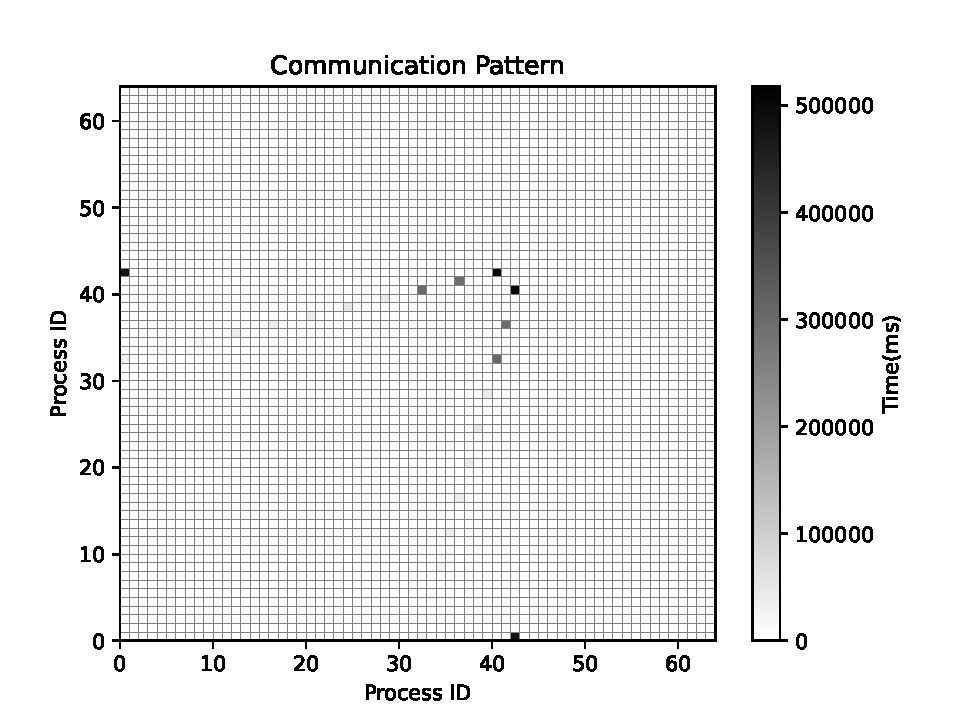
\includegraphics[width=0.23\textwidth]{comm_pattern/dt.B.pdf}
  }
  \subfigure[FT]{
    \centering
    \includegraphics[width=0.23\textwidth]{comm_pattern/ft.B.pdf}
  }
  \subfigure[IS]{
    \centering
    \includegraphics[width=0.23\textwidth]{comm_pattern/is.C.pdf}
  }
  \subfigure[LU]{
    \centering
    \includegraphics[width=0.23\textwidth]{comm_pattern/lu.B.pdf}
  }
  \subfigure[SP]{
    \centering
    \includegraphics[width=0.23\textwidth]{comm_pattern/sp.B.pdf}
  }
  \subfigure[SWEEP3D]{
    \centering
    \includegraphics[width=0.23\textwidth]{comm_pattern/sweep3d.pdf}
  }
\end{figure}


\section{进程相似性分析}

使用\perflow{}实现进程相似性分析的分析任务,在NPB基准测试程序和SWEEP3D上进行测试。测试结果如下:

\begin{figure}[!htb]
  \centering
  % \includegraphics[width=0.9\textwidth]{}
  \subfigure[BT]{
    \centering
    \includegraphics[width=0.3\textwidth]{procs_similarity/bt.B.pdf}
  }
  \subfigure[CG]{
    \centering
    \includegraphics[width=0.3\textwidth]{procs_similarity/cg.B.pdf}
  }
  \subfigure[DT]{
    \centering
    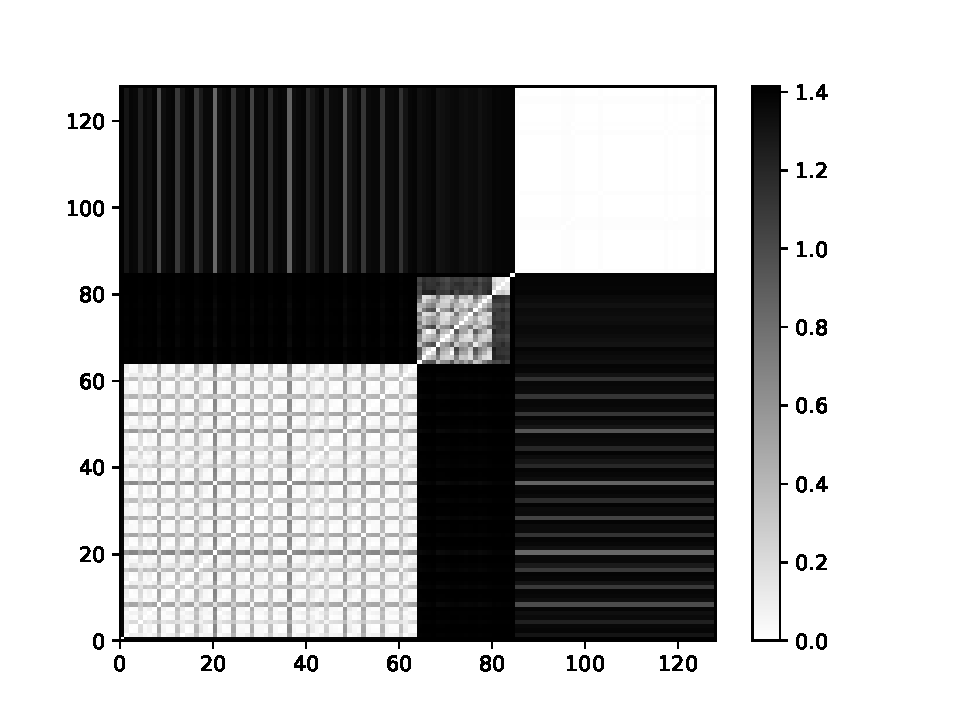
\includegraphics[width=0.3\textwidth]{procs_similarity/dt.C.pdf}
  }
  \subfigure[EP]{
    \centering
    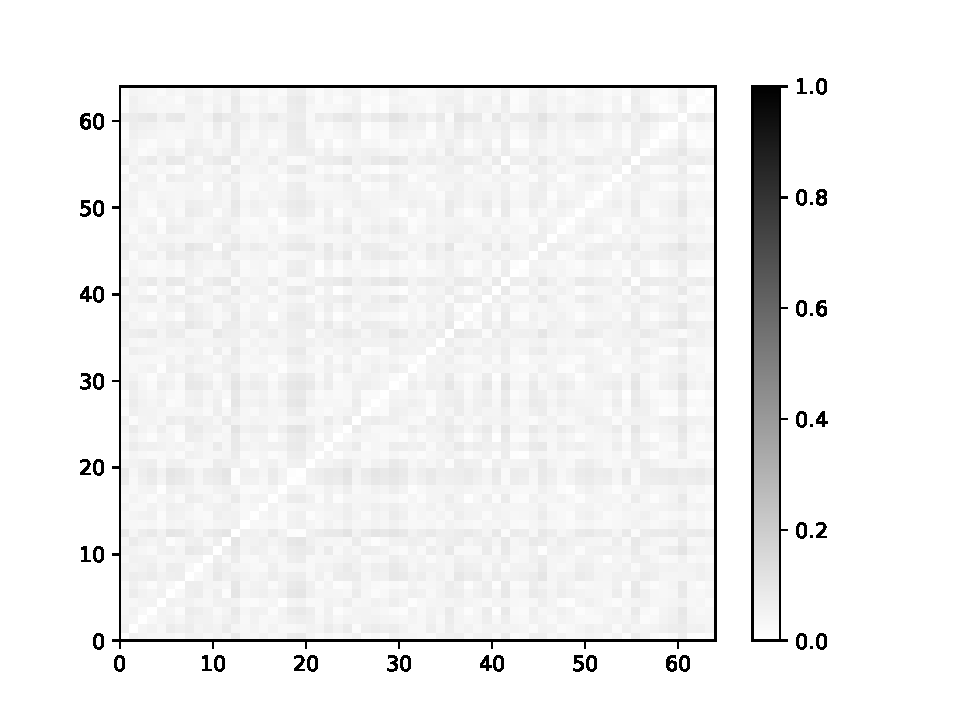
\includegraphics[width=0.3\textwidth]{procs_similarity/ep.C.pdf}
  }
  \subfigure[FT]{
    \centering
    \includegraphics[width=0.3\textwidth]{procs_similarity/ft.B.pdf}
  }
  \subfigure[IS]{
    \centering
    \includegraphics[width=0.3\textwidth]{procs_similarity/is.C.pdf}
  }
  \subfigure[LU]{
    \centering
    \includegraphics[width=0.3\textwidth]{procs_similarity/lu.B.pdf}
  }
  \subfigure[SP]{
    \centering
    \includegraphics[width=0.3\textwidth]{procs_similarity/sp.B.pdf}
  }
  \subfigure[SWEEP3D]{
    \centering
    \includegraphics[width=0.3\textwidth]{procs_similarity/sweep3d.pdf}
  }
\end{figure}


% \nocite{*}
% \printbibliography[heading=bibintoc, title=\ebibname]

\appendix
%\appendixpage
\addappheadtotoc

\end{document}
